% A simple template for LaTeX documents
% 
% To produce pdf run:
%   $ pdflatex paper.tex 
%


\documentclass[12pt]{article}

% Begin paragraphs with new line
\usepackage{parskip}  

% Change margin size
\usepackage[margin=1in]{geometry}   

% Graphics Example:  (PDF's make for good plots)
\usepackage{graphicx}               
% \centerline{\includegraphics{figure.pdf}}

% subfigures, side by side
\usepackage{subcaption}

% hyperlinks
\usepackage{hyperref}

% Blocks of code
\usepackage{listings}
\lstset{basicstyle=\ttfamily, title=\lstname}
% Insert code like this. replace `plot.R` with file name.
% \lstinputlisting{plot.R}

% Monospaced fonts
%\usepackage{inconsolata}
% GNU \texttt{make} is a nice tool.

% Supports proof environment
\usepackage{amsthm}

% Allows writing \implies and align*
\usepackage{amsmath}

% Allows mathbb{R}
\usepackage{amsfonts}

% Numbers in scientific notation
% \usepackage{siunitx}

% Use tables generated by pandas
\usepackage{booktabs}

% Allows umlaut and non ascii characters
\usepackage[utf8]{inputenc}

% norm and infinity norm
\newcommand{\norm}[1]{\left\lVert#1\right\rVert}
\newcommand{\inorm}[1]{\left\lVert#1\right\rVert_\infty}

% Statistics essentials
\newcommand{\iid}{\text{ iid }}
\newcommand{\Exp}{\operatorname{E}}
\newcommand{\Var}{\operatorname{Var}}
\newcommand{\Cov}{\operatorname{Cov}}


%%%%%%%%%%%%%%%%%%%%%%%%%%%%%%%%%%%%%%%%%%%%%%%%%%%%%%%%%%%%

\begin{document}

\title{Code Analysis Project Proposal}
\date{\today}
\author{Clark Fitzgerald}
\maketitle

\begin{abstract}

\end{abstract}

\section{Introduction}
%%%%%%%%%%%%%%%%%%%%%%%%%%%%%%%%%%%%%%%%%%%%%%%%%%%%%%%%%%%%

The idea behind code analysis is to treat the code itself as a data
structure as ``Programming on the language'' opens up rich possibilities.
This is an old idea, both the R and Julia language references cite Lisp
as the inspiration \cite{Rlang} \cite{bezanson2014julia}.

Compilers have used all manners of static analysis and
intermediate optimizations to create more efficient code. Interpreted
languages are much more limited in this respect. This project explores
the use of an alternative evaluation model to improve performance while
preserving language semantics.

The evaluation model for interpreted languages is simple. Each
expression of code is evaluated in the order that it appears. Informally
each expression is a line of code. This can be
viewed as a set of constraints on the evaluation order of the expressions:
\begin{enumerate}
    \item expression 1 executes before expression 2
    \item expression 2 executes before expression 3
    \item $\dots$
\end{enumerate}
What if these constraints are relaxed? Suppose expression 1 defines the variable
\texttt{x}, which is not used until expression 17. Then one has the
constraint:
\begin{enumerate}
    \item expression 1 executes before expression 17
\end{enumerate}
This can be generalized into a directed graph by considering expressions as
nodes and constraints as edges. The edges are implicit based on the order
of the statements in the code. Add an edge from $i \rightarrow k$ if
expression $k$ depends on the execution of expression $i$.  It's safe to
assume $i < k$, because expressions appearing later in a program can't
affect expressions which have already run. Hence the expression graph is
acyclic, ie. a DAG.

Scheduling execution based on the expression graph allows some expressions to execute in
parallel. For example, the following adjacent lines are independent, so
they can be computed simultaneously:

\begin{verbatim}
sx = sum(x)
sy = sum(y)
\end{verbatim}

Mathematically, the standard evaluation model is a total ordering on the
set of expressions in the code. The dependency graph is a partial ordering.

On a broader note, this is about embedding more intelligence into the 
system. Many languages have mechanisms or third party tools for explicitly
requesting asynchronous evaluation. These typically require changing the
code. This introduces complexity, makes maintenance more difficult, and
makes the code less portable.  It's more convenient to have one version of
the code which can be passed to a system which will just ``do the right
thing'', adjusting to different platforms, work loads, and data sizes on
the fly. 

\section{Literature Review}
%%%%%%%%%%%%%%%%%%%%%%%%%%%%%%%%%%%%%%%%%%%%%%%%%%%%%%%%%%%%

The expression graph proposed above is similar to 
use-definition and definition-use chains. A definition-use chain consists
of all expressions using a variable following the definition of that
variable. This amounts to a subset of the edges in the expression graph,
since it's possible that expressions depend on each other without
variables. For example, consider the following R code to save a plot to a
pdf:
\begin{verbatim}
pdf("xy.pdf")
plot(x, y)
title("x and y")
dev.off()
\end{verbatim}
These expressions depend on each other, but only \texttt{plot(x, y)} uses variables.

The Use-definition chain has been around since at least 1978
when it was used to remove dead (unused) code \cite{kennedy1978use}.
Code usefulness is defined recursively; a computation is useful if the result is
used later by another computation. This is combined with the ``base case''
of usefulness, a set of operations considered
intrinsically useful. This author considers calls to subroutines and branch
test instructions as intrinsically useful. We might take this idea and
tweak it a little- define expressions in a data analysis script as
intrinsically useful if they have a side effect, for example
saving data to disk.

More general than the use-definition chain is the program dependence graph (PDG)\cite{ferrante1987}:
\begin{quote}
    A PDG node represents
    an arbitrary sequential computation (e.g., a basic block, a
    statement, or an operation). An edge in a PDG represents
    a control dependence or a data dependence. PDGs do not
    contain any artificial sequencing constraints from the
    program text; they reveal the ideal parallelism in a
    program. \cite{sarkar1991automatic} 
\end{quote}
\cite{sarkar1991automatic} goes on to make the practical distinction between ideal
parallelism and useful parallisism. Overhead implies that the two often
differ.
The expression graph differs from the PDG since it allows the permutation of
operations in a basic block.

The hierarchical task graph (HTG) was introduced in \cite{girkar1992automatic}
to detect task parallelism in source code for use in compilers.
As in the others, it incorporates the control flow for a fine grained
parallelism. They allow `compound nodes' containing nested HTG's.
\cite{cosnard1995automatic} describe constructing a task graph based on
annotating the source code the program.
\cite{adve2004parallel} presents a model for predicting the run time of
programs based on a task graph. 

The literature cited in this section focuses primarily on compiled
languages along with careful analysis of control flow. Most examples and
applications presented along with these papers are for well-defined
algorithmic problems. These algorithmic problems are often quite different
than a high level data analysis script which may call down into several
different algorithms.

\section{Languages Requirements}
%%%%%%%%%%%%%%%%%%%%%%%%%%%%%%%%%%%%%%%%%%%%%%%%%%%%%%%%%%%%

We can consider building the expression graphs described above for languages that are
\begin{itemize}
    \item open source
    \item used for data analysis
    \item high level
    \item interpreted
    \item enable metaprogramming
\end{itemize}
Metaprogramming warrants more explanation. This refers to programmatically
inspecting and potentially modifying code from within the language.  It is
needed to determine when variables are created and used, among other
things.  The current popular languages satisfying these requirements are
Python, Julia, and R.

The basic unit to analyze is a single code expression.
Consider how an expression uses symbols, aka variables or names.
An expression may do any combination of the following things:
\begin{enumerate}
    \item Define new symbols: \texttt{x = 10}
    \item Use existing symbols: \texttt{sin(x)}
    \item Redefine existing symbols: \texttt{x = 20}
\end{enumerate}

\begin{table}[]
\centering
    \caption{Sorting \texttt{x} in place}
\label{tab-sort}
\begin{tabular}{ll}
    \textbf{language} & \textbf{code}        \\
\hline
    Python   & \texttt{x.sort()}    \\
    Julia    & \texttt{sort!(x)}    \\
    R        & \texttt{x = sort(x)}
\end{tabular}
\end{table}

Consider sorting a numeric vector as in Table \ref{tab-sort}.
The Julia and Python methods modify their arguments in place.  From a
computational standpoint this is great, since it allows the implementations
to use more space efficent sorting techniques. However, from a code
analysis standpoint this behavior is undesirable, since it means that we
need to assume generally that every method call in these languages both
uses and updates the object. Since data analysis scripts mainly consist of
function and method calls this will excessively contrain the problem.

It may be possible to recursively examine all functions and methods which
are used, but this is not ideal for a couple reasons. First, it would
require analyzing the underlying library code, which is orders of magnitude
more code than what the user has written. Second, eventually we'll get to
compiled code which requires totally different methods. For example, LLVM
can be used to programmatically generate use-definition chains
\cite{lattner2004llvm}.

Hence functional programming and pass by value semantics make constructing
graphs much more feasible. The R language is ideal in this respect.

\section{Related Work}
%%%%%%%%%%%%%%%%%%%%%%%%%%%%%%%%%%%%%%%%%%%%%%%%%%%%%%%%%%%%

Jim Hester's covr package \cite{R-covr} checks unit test coverage of R
code. It is a practical example of computing on the language,
programmatically modifying the code by recording calls as they are made.
He pointed out a nice relevant idea distinguishing between AST's, parse
trees, and "lossless syntax trees":
\url{https://news.ycombinator.com/item?id=13628412}. To inject code into a
script one needs to be very
careful to preserve structure lost after parsing, ie.
comments and formatting. This is a non-trivial task.

A similar strategy of recording calls should work to collect timings and
resource usage for functions called with various data sizes. This could be
implemented with something like \texttt{System.time()}. This would allow us
to time each expression. Then we can potentially use this to change the
execution: ie. if $n > 1000$ then run a multicore version. This resembles
something like Profile Guided Optimization (PGO). 

Maybe a simpler way to do this is to just use the built in profiler. Use
the results to determine whether parallelization is worth it, and maybe set
some bounds for expected performance changes if one uses various forms of
parallelism. 

There may be potential to use statistical methods for this.
Run it many times, collecting profiling results for various values and use
this as the training data. After all, we have easy access to all the
machine learning type things that we need. We can use it to automatically
tune. But this implies that there is some way to tune it. Right now the
only "trick" I have up my sleeve is to try to parallelize it.

The vignette in Tierney's \texttt{proftools} package has some nice examples
of visualizing profiling data \cite{R-proftools}. The call graphs and related visualizations
are conceptually similar to what might be done with the expression graph.
\texttt{profvis} integrates with the IDE to indicate the actual
line of source code along with the related timing info \cite{R-profvis}.

Xie's \texttt{knitr} facilitates reproducible computations for
chunks of code in Rmarkdown documents \cite{R-knitr}. One feature it enables is caching,
ie. it doesn't need to run a chunk of code if nothing has changed. One can
manually specify the chunk dependencies by relative or absolute indices,
ie. -2 for the chunk 2 blocks in front of the current chunk, or 1 for the
first chunk. This seems unreliable because it requires the user to
accurately infer the dependency information, and it doesn't automatically
adjust if one inserts new chunks in the document.

Knitr also has an \texttt{autodep} option to infer this dependency
information. This works by comparing the global variables existing before
and after running the code in each chunk. It stores this information in
special files. So it doesn't use any static analysis of the code.

But the structure of knitr blocks here is actually very appealing- this is
a great use case for the parallelism. Why not evaluate the chunks in
parallel if possible? I wonder how difficult it would be to hook into
knitr's system... And while I'm at it, why not Jupyter Notebooks? If I can
figure out how to build an equivalent code dependency graph for Python that
is.

Henrik Bengston's \texttt{future} package provides a mechanism for
asynchronous evaluation of R expressions \cite{R-future}. Once the
expression graph is created it might be possible to use this for
evaluation.

\section{Graph Construction}
%%%%%%%%%%%%%%%%%%%%%%%%%%%%%%%%%%%%%%%%%%%%%%%%%%%%%%%%%%%%

To start off we make two assumptions on the program. First it's assumed to
be correct, meaning that it will run sequentially without errors.
Second every expression should be strictly necessary. This can be achieved
through a preprocessing step removing dead code.

The expression graph and related data structures are related to the parsed
script, referred to as the \textbf{parse tree}. The expression
graph is a function of the parse tree. Since the parser
doesn't care about non significant white space and comments,  different
scripts can produce the same parse tree.  Many parse trees can give rise to
the same code graph. For example, the expression graph shouldn't care if one uses
\texttt{=} or \texttt{<-} for assignment. Nor will it care about the
ordering of two adjacent lines binding a symbol to a literal constant:

\begin{verbatim}
a = 1
b = 2
\end{verbatim}

Therefore we lose information by converting from a parse tree to an
expression graph.

We can also introduce an artificial (graph style) source and sink representing the
beginning and end of the program, respectively.

Figures \ref{fig:ast} and \ref{fig:codegraph} illustrate the ideas of
a parse tree an expression dependency
graph for the four lines of code in listing \ref{list:ab}.  Edges 1 and 3
represent the respective uses of the variable \texttt{n} and \texttt{x}.
Edge 2 comes from the redefinition of \texttt{n}.  Edge 5 propagates the
most recent definition of \texttt{n}.  The least obvious is edge 4, which
is necessary to respect R's lexical scoping semantics since \texttt{x <-
rnorm(n)} uses the first definition of \texttt{n}. The general rule here is
that all statements using one version of \texttt{n} must execute before
\texttt{n} can be redefined.

The dashed edges in \ref{fig:codegraph} are redundant for representing
expression dependence given the other edges. Indeed, the code in
listing \ref{list:ab} must run sequentially. One may wish to remove such
redundant edges, especially for visual presentation of a larger program.

\lstinputlisting[language=R, caption=Simple script, label=list:ab]{../experiments/ast/ab.R}

\begin{figure}
\centering
\begin{subfigure}{.6\textwidth}
    \centering
    \includegraphics[width=.8\linewidth]{../experiments/ast/ast.pdf}
    \caption{Parse tree}
    \label{fig:ast}
\end{subfigure}%
\begin{subfigure}{.4\textwidth}
  \centering
  \includegraphics[width=.8\linewidth]{../experiments/ast/codegraph.pdf}
  \caption{Expression dependency graph}
  \label{fig:codegraph}
\end{subfigure}
\caption{Different representations of the script in Listing \ref{list:ab}}
%\label{fig:test}
\end{figure}

The existence of some edges may depend on conditional statements which can't
be known until run time. In this case the conservative and correct way to
handle the situation is to add the edges in question. For example, in the
following code one assumes that the expression \texttt{x <- 10} will run.

\begin{verbatim}
# coinflip() randomly returns TRUE or FALSE
if(coinflip()){
    x <- 10
}
\end{verbatim}

\section{Task Based Parallelism}
%%%%%%%%%%%%%%%%%%%%%%%%%%%%%%%%%%%%%%%%%%%%%%%%%%%%%%%%%%%%

It's reasonable to try to improve code performance if slow speed affects
many users. For scripts, superficially it might appear that few people are
affected. Indeed, if a researcher writes one script that takes a couple
minutes to run, and they run it a couple times then it doesn't matter much,
and there's no point in attempting to accelerate it.  However, these same
sorts of "scripts" can be used in more serious ways.  For example, scripts
can be used as Extract Transform Load (ETL) tools that run as batch jobs
every day or every hour. Then the script runs many times, so it's important
to realize more performance. For ease of use and maintainability it's nice
to have automatic tools to accelerate the performance. One can write
natural, beginner level scripts and have them run much faster.

As of 2009, most efforts to parallelize R have focused on the lower level
programming mechanisms \cite{schmidberger2009state}. These needed to be in
place before any higher level automatic detection could be built and
function.

Let $k$ be the number of cores on a machine.
To accelerate code using this single machine the best possible case is if
we can keep all $k$ cores busy at once. This will happen if there are $nk$
expressions which can be independently scheduled for some positive integer
$n$. 
On a two core machine that script might look something like:

\begin{verbatim}
# These could be run in parallel
a = long_running_func()
b = long_running_func()
\end{verbatim}

The worst possible case is if the second long running computation depends
on the first, and everything else depends on the second. Then it must run
in serial so parallelism can't help.

\begin{verbatim}
a = long_running_func()
b = long_running_func2(a)  # depends on a
# Now perform many operations on b
\end{verbatim}

\subsection{Static Execution}
%%%%%%%%%%%%%%%%%%%%%%%%%%%%%%%%%%%%%%%%%%%%%%%%%%%%%%%%%%%%

If overhead and expression run time are approximately known then the
question of optimal execution for the complete expression dependency graph
can be framed as a scheduling optimization problem and solved statically.
The objective function to minimize is the total wall clock time to complete
execution. Constraints come from the depenedency graph and that at most $k$
cores may be active at one time.

To consider an alternative evaluation model the overhead required to
parallelize an expression should require less time than running the
expression itself. Rounding to orders of magnitude, here are some rough
times for reference executing on a modest machine. Simple R expressions
take $10^{-7}$ seconds to evaluate. Using a system level parallel fork
requires $10^{-3}$ seconds of overhead. Evaluation on an existing local
socket cluster takes $10^{-4}$ seconds. Then either of these well
established methods for parallelism in R won't become efficient until the
code under evaluation takes on the order of $10^{-3}$ seconds.
These timings include latency for interprocess communication on a single
machine. Bandwidth is also an issue, since serializing large amounts of
data between processes, ie. millions of floating point numbers, will impact
performance. For example, listing \ref{list:overhead} squares each element
of a vector of one million floating point numbers. Memory transfer overhead causes
a parallel evaluation to take more than an order of magnitude more time
than the regular version. 
Technical solutions such as threading and shared memory have the
potential to reduce these sources of overhead.

\lstinputlisting[language=R, caption=Overhead caused by memory transfer,
label=list:overhead]{overhead.R}

Issues of latency and bandwidth generally become more complex for different
architectures such as distributed systems and GPU's.


\subsection{Dynamic Execution}
%%%%%%%%%%%%%%%%%%%%%%%%%%%%%%%%%%%%%%%%%%%%%%%%%%%%%%%%%%%%

Alternatively a dynamic execution model can be used that .
Thinking about how to run the whole thing in parallel now. I could use a
model where the master sends out expressions to workers to
evaluate. This would be through an event loop that pops expressions from a data
structure.

And forks every time. Then the master polls the workers to see
when they're finished. Though it would be better if the workers could send a
message saying when they're finished. Seems like I might be able to do this
with \texttt{parallel::sendMaster}.

The process forking every time will be quite inefficient. The more intelligent
thing to do is `pipeline' the operations, and send whole related blocks of
expressions to various processes to evaluate.

The processes spawned with \texttt{parallel::mcparallel} communicate
through an OS level pipe aka FIFO. This is why the function returns a vector of
length 2 called `fd` for file descriptor, among other things. These are the
file descriptors to the pipes

But this may open up a different opportunity for faster, lighter weight
threads? A main consideration with threads is that one doesn't want one
thread to mess up a the data structure while another is using using it. But
perhaps using this expression dependency information will let us make
guarantees about safety?

Or what about using something even lighter than threads- like coroutines or
callbacks? It might be possible to dig into the guts of R and make
something like this.

This approach is different than rewriting the script as I did before. It's appealing
because it can do dynamic load balancing.

But it's not clear which expressions to evaluate first. Maybe I should
first do the ones that have the most dependencies? If an expression has no
dependencies then one can do it at any time, even way later. But if there
are many dependencies then none of them can run until the parent is
evaluated. This will end up needing some data structure acting like a priority queue.

Here's an algorithm: Start by marking all direct descendants of the special
0 (start) node as ready. Let the workers begin evaluating these
expressions.

\begin{enumerate}
    \item Expression $e_i$ is evaluated and the results are available again
        on master.
    \item For each expression $e_j$ which depends directly on $e_i$: check
        if $e_j$ has no other existing parents then mark it as ready.
    \item Remove $e_i$ from the graph.
    \item Worker begins executing any of the nodes that are marked as ready.
\end{enumerate}

There's some nuance here by trying to keep each of $k$ workers as busy as
possible while still respecting the constraints. Ie. there may be
bottlenecks where only one worker can be active, but after that all the
others can go.

This algorithm could also be refined into a priority queue by keeping the ready
nodes in a heap, with the values determining the heap order as the number
of expressions that depend on that expression, directly or indirectly. This
is a little naive- it would be better to have timings of the code and do
something more optimal in terms of reducing run time.


\section{How CodeDepends works}
%%%%%%%%%%%%%%%%%%%%%%%%%%%%%%%%%%%%%%%%%%%%%%%%%%%%%%%%%%%%

The parsing uses an object oriented wrapper around R's builtin \texttt{parse()}
which handles different file types ie. script or dynamic documents among other arguments.
This doesn't directly expose code comments.
At first glance it seems CodeDepends uses the tokens
more indirectly, through functions like \texttt{is.name()}. 

The workhorse functions are in \texttt{CodeDepends.R}. Overall, the
approach resembles \texttt{codetools::walkCode} as discussed in
\ref{chambers2016extending}. Essentially it walks the tree of code, calling
a function to collect usage information.

When analyzing a single expression, first a 
collector object is created with \texttt{inputCollector()}. This is a
closure that maintains a list of everything in the expression that has been seen
so far: files, variables, function calls, etc. It returns a list of
functions to update the data in the closure.

\texttt{getInputs.language()} takes a collector object and
recurses through expressions until it finds the leaf nodes which can be functions, calls, assignments,
names, literals, or pairlists. Upon finding one of these leaf nodes it
calls the collector object. 
Many special cases of functions are handled in functionHandlers.R, such as
\texttt{\$, rm, for} as well as non standard evaluation. Special attention seems
to have been paid to dplyr operations.

As a user I'd like a clean, well defined entry point and API for this
stuff. The problem I had today was trying to pass arguments into
\texttt{inputCollector}. I did this by hacking through the code of
\texttt{makeTaskGraph}.

TODO: Ask Duncan where the separation between CodeDepends and CodeAnalysis
should be. How about makeTaskGraph? Probably first I should just look more
in CodeAnalysis to see what's there.

The \texttt{ScriptNodeInfo} objects contain all processed information about
each expression. They tell which variables 


\section{Applications}
%%%%%%%%%%%%%%%%%%%%%%%%%%%%%%%%%%%%%%%%%%%%%%%%%%%%%%%%%%%%

What are all the useful things to do when rewriting code?  Duncan's very
helpful docs here http://www.omegahat.net/CodeDepends/design.pdf give a
handful of reasons.

Other things that I can think of:

Identification and elimination of dead code.

- Given a big ugly script, pull out the minimal set of code to produce a
  final result. For example, everything needed to make `plot(finalresult)`.
- Parse Rhistory to find the minimal set of code to reproduce a result.
- Separate single scripts into multiple scripts if they actually have two
  independent sequences of computation.

These ideas stay much closer to the syntax and language of R compared to
what Nick is doing.

I've been considering this for the purpose of analyzing, accelerating and
optimizing essentially single scripts. But how important is this generally?
It only matters if someone's script runs slow. Probably this mostly happens
due to one large computation. If they're doing two large and independent
computations in one script shouldn't that be two scripts? But these tools
should be able to split them up at that level if I ask them to.

Remove all objects as soon as they're finished being used in the script. If
creating many large intermediate objects this could help with not using
excessive memory.

\section{Detecting Parallelism}
%%%%%%%%%%%%%%%%%%%%%%%%%%%%%%%%%%%%%%%%%%%%%%%%%%%%%%%%%%%%

Not sure how to generally detect where the possibilities for
parallel are. In a simple case of k obvious threads with one common
ancestor and common child there is an obvious option:

Remove the common ancestor and child and select the k disjoint subgraphs
between them.

Alternatively:

1. Start at the top of the graph, and move down until one node has
multiple children. Gather those child threads into 2 groups.
2. Same thing starting at the bottom.

The most straightforward thing to do right now is take a more complex
graph, say something like this:

\centerline{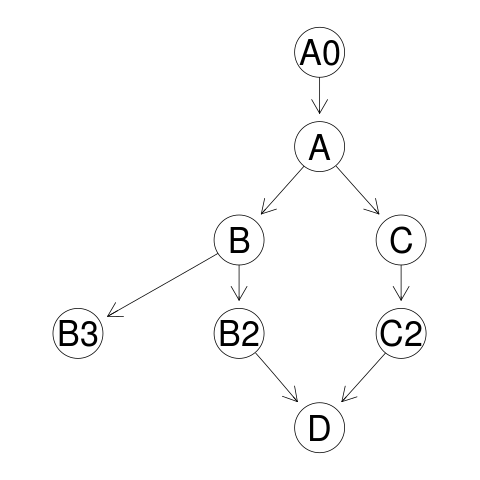
\includegraphics{../codedepends/larger_graph.png}}


And attempt to collapse the structure into one where the parallel threads
become obvious:

\centerline{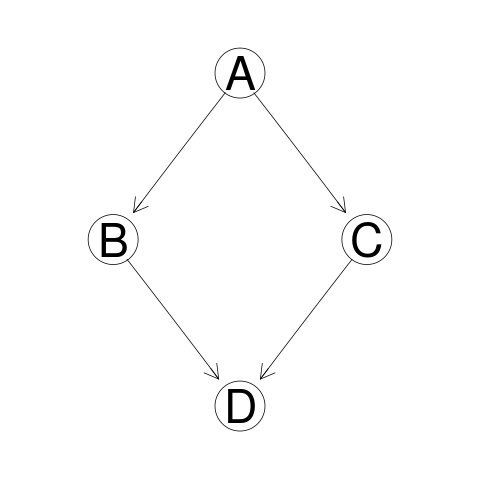
\includegraphics{../codedepends/simple_graph.png}}

The essential part for the multiprocessing is to have many "adjacent"
threads (is there a correct graph term for this?)
Optionally the adjacent threads can share a common parent and or child
nodes.

\section{Hard things}
%%%%%%%%%%%%%%%%%%%%%%%%%%%%%%%%%%%%%%%%%%%%%%%%%%%%%%%%%%%%

`fit = lm(y ~ x)` doesn't detect the dependency of `fit` on `x, y`.

Following the control flow for `lm` we see the following calls:
`model.matrix.lm`, `model.frame.default`, `as.formula`. But eventually this
`y ~ x` itself must be evaluated in which case `.Primitive("~")` is called,
which certainly does something weird. But what?

Haven't yet checked things like:
`<<- assign`

Recursion? Iterating updates?

Random number generation across processes. I'll need to make sure that it's
possible to reproduce random things. In general it's not going to be the
same if it's single threaded or multithreaded, but this is true in general,
so I don't need to worry about it.

\begin{quote}
     The behaviour with ‘mc.set.seed = TRUE’ is different only if
     ‘RNGkind("L'Ecuyer-CMRG")’ has been selected.  Then each time a child
     is forked it is given the next stream (see ‘nextRNGStream’).  So if
     you select that generator, set a seed and call ‘mc.reset.stream’ just
     before the first use of ‘mcparallel’ the results of simulations will
     be reproducible provided the same tasks are given to the first,
     second, ...  forked process.

     -R documentation for parallel::mcparallel
\end{quote}

I'll need to think carefully about what happens with dynamic evaluation.
And a related idea, functions can use variables that don't yet exist- but this
is weird- I just need to preserve the correct order. Here's some examples:

\begin{verbatim}
f = function() 0        # 1
g = function() f() + 1  # 2
f = function() 10       # 3
g()                     # 4
\end{verbatim}

The last line returns 11, since it uses most recent version of f().
The current dependency graph imposes this partial order:

\begin{verbatim}
1 -> 2, 1 -> 3, 2 -> 4
\end{verbatim}

So the statements could be written in the following order while still respecting the
partial order:

\begin{verbatim}
f = function() 0        # 1
g = function() f() + 1  # 2
g()                     # 4
f = function() 10       # 3
\end{verbatim}

In this case the call to g() will incorrectly return 1 instead of 11.
Hence there is a ``hidden'' dependency implicit here: \texttt{3 -> 4}.

TODO: Cite Nick's SSA reference.

A couple ideas to get around this: inline functions defined in the script.
Think harder about when evaluation must happen.

\section{Scripts in the Wild}
%%%%%%%%%%%%%%%%%%%%%%%%%%%%%%%%%%%%%%%%%%%%%%%%%%%%%%%%%%%%

I could do some analysis on scripts that I scrape to determine theoretical
bounds for the number of statements that must be run sequentially,
and the max number of concurrent workers. My example script I've been
working on has about 50 statements, and I think min number of sequential
statements is around 10. Need to check. This could motivate reducing
overhead though.

Duncan suggests to find R code that's unacceptably slow, and see what these
methods can do to improve it. So to get a better sense of theoretical
improvements I could execute the code in normal R and attach timings for
each expression. This would show me true lower bounds for the method. It
would also be quite interesting to have some sense of the distribution of
execution times for different types of code. I imagine it varies
dramatically, but there may be rough patterns. One result I'm expecting is
that just one or two lines dominate the total script run time. In which
case anything I do can't really help. Unless that line calls one function
and I can use this method on the one function.

Vignettes, including those found on bioconductor, are for instructional
purposes, so they're mostly simple and self contained. This isn't the use
case I'm targeting. They are nice because the data should be included with
the package, thus I have some hope of actually being able to run them if
needed.

To get some idea of the potential for speedup, if I have an unlimited
number of cores, no overhead, and each expression takes roughly the same
amount of time to execute then the script can run no faster than the length
of the longest path in the graph. Hence speedup will be the total number
of statements divided by the length of the longest path in the graph.
By the way, all of those assumptions are unreasonable.



\section{Implementation}
%%%%%%%%%%%%%%%%%%%%%%%%%%%%%%%%%%%%%%%%%%%%%%%%%%%%%%%%%%%%

At first I iterated over the blocks of code and gathered dependency info as
I went along. But then I switched the implementation to focus on the variables
themselves to make my code easier to reason about. It should be slightly
more efficient, but that's not really a concern yet.

I consider updates of a list to be changes to the global list variable.
Thus something like the following redefines x every time. 

\begin{verbatim}
    x = list()
    x$a = f(...)
    x$b = g(...)
\end{verbatim}
 
This is easy and safe to do, but it might be inefficient if \texttt{f, g}
are expensive functions, because they could be run in parallel. An
alternate way is to think of \texttt{x\$a} as a variable that depends on
the original \texttt{x}. But adding details like these isn't worth it to me
now, because it's not core to what I'm trying to accomplish.

Detail- Calls to \texttt{library} need to make it to the top of the graph. Maybe in
general I can adopt the \LaTeX idea of a preamble, or setup code. But what else would go
there besides library?

It would be nice if I could look at the R global environment, then
look at an updated environment after running a line of code and take this
as the update. 

\newpage
\newpage

\section{Chunking}

IDEA: nested parallelism- how to do it? If you hard code it in you're
stuck.

The task based parallelism isn't as relevant to how people use R (and other
languages) for data processing. Instead
lets think more about chunking and data parallelism. 

Parallelism introduces additional overhead on top of what dynamic languages
already incur. A general strategy to minimize this overhead is to ``chunk''
the computations. For example, given 1000 parallel operations one might
partition these into chunks of size 100 so that they become 10 parallel
tasks \cite{matloff2015parallel}.

I can take the code in \cite{matloff2015parallel} and see how changing the
chunk sizes affects the run time. I could also do this with Python's dask.
The goal is to draw general conclusions about which chunk sizes work best
based on the amount of computation.

It would be nice to run just a couple in serial on the master process and
make principled decisions about how to run based on these results. For
example:
\begin{itemize}
    \item Is it worth it to run in parallel?
    \item Should we chunk? What should the chunk sizes be?
    \item Reverse the order for better load balancing?
    \item Dynamic or static scheduling?
\end{itemize}

Usually none of these are known ahead of time.  They also depend on the
particular problem.  The only way to know if a chunking scheme will work is
to experiment with a similar problem, then check expectations for the next
one. I also expect that they vary across different machines.

The book mentions using large chunks in the beginning followed by small
chunks for superior load balancing.

Programming in the RDSM package conceptually is very similar to OpenCL on
the GPU. You allocate memory and send it to the workers, then update it in
place based on thread IDs. This is quite different than normal functional
R. I wonder if we could "translate" regular R into this style of
programming?

TODO: Come up with application where I need all this!! How about computing
graphs from Euclidean space like with James' application? It would be nice
for the QE to have something that he's familiar with and invested in.

\appendix
\section{LLVM}

LLVM has some functionality for working with these use / def chains
\cite{Lattner2004}. For example:
\url{http://llvm.org/docs/ProgrammersManual.html#iterating-over-def-use-use-def-chains}.
Following their terminology, an object of class \texttt{Value} is used by
potentially many objects of class \texttt{User}. The \emph{def-use} chain
is the list of all \texttt{Users} for a particular \texttt{Value}. I think
of this as all the places in the code where this variable propagates. In
contrast, the \emph{use-def} chain is the list of all \texttt{Values} for a
particular \texttt{User}. This is all the inputs to a newly
created object. There's room for both of these chains to be expanded recursively.

In this example the def-use chain for \texttt{x} is only \texttt{[y]}, but the
recursive one is \texttt{[y, z, z2]}. The use-def chain for \texttt{y} is
\texttt{[z, z2]}.

\begin{verbatim}
x = 10
y = x + 5
z = y + 2
z2 = y + 100
\end{verbatim}

We might be able to use this along with R code to determine if an R
function calling C code is pure.

\appendix
\section{Definitions}
%%%%%%%%%%%%%%%%%%%%%%%%%%%%%%%%%%%%%%%%%%%%%%%%%%%%%%%%%%%%

We need to start out with some definitions and basic concepts to make all
of this precise. The following material is from the R
Language Reference \cite{Rlang}.

``A \textbf{statement} is a
syntactically correct collection of tokens.'' Less formally one can think of
a statement as a single line of code. The `line' rule doesn't always hold in practice,
since a semicolon can put two statements on one line, and a single
statement may span multiple lines.

\begin{verbatim}
# Two statements on line
a = 1; b = 2

# One statement on multiple lines
plot(x,
     y)
\end{verbatim}

\textbf{symbol} is a variable name such as \textbf{a, b} above.  The words
symbol, variable, and name are used interchangeably. For consistency I'll
stick with symbol.

Assignment is the binding of a symbol to an R object.

``An \textbf{expression} contains one or more statements.'' Expression objects
in the langauge contain parsed but unevaluated statements. 

Statements can be grouped together using braces to form a \textbf{block}.
Since expressions can be nested, we can consider a block just a special
type of expression.

\begin{verbatim}
{
a = 1
b = 2
}
\end{verbatim}



\bibliographystyle{plain}
\bibliography{citations} 

\end{document}
